\documentclass[tikz]{standalone}
\usepackage{pgfplots}
\pgfplotsset{compat=1.15}
\usepackage{mathrsfs}
\usetikzlibrary{arrows,calc}
\usepackage{tkz-euclide}
\pagestyle{empty}

\definecolor{AngleClr}{rgb}{0,0.39215686274509803,0}
\definecolor{ShapeClr}{rgb}{0.6,0.2,0}

\begin{document}

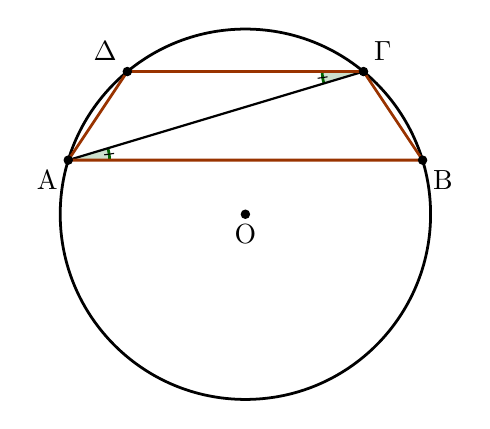
\begin{tikzpicture}[scale=.75]
\tkzSetUpLine[line width=1pt,color=black]
\tkzSetUpPoint[fill=black]

\tkzDefPoints{0/0/A,6/0/B,1/1.5/D,5/1.5/C}

\tkzDefPointBy[projection=onto C--D](A)\tkzGetPoint{A'}
\tkzDefPointBy[projection=onto C--D](B)\tkzGetPoint{B'}

\tkzDefCircle[circum](A,B,C) \tkzGetPoint{O}
\tkzFillPolygon[fill=white](A,B,C,D) 

\tkzFillAngles[fill=AngleClr,size=.7,fill opacity=0.2](D,C,A B,A,C)
\tkzMarkAngles[line width=1pt,color=AngleClr,size=.7,mark=|,mksize=1.8](D,C,A B,A,C)


\tkzDrawCircle[line width=1.0pt, color=black](O,A)

\tkzDrawSegment[line width=0.8pt](A,C)

\tkzDrawPolygon[color=ShapeClr](A,B,C,D)
\tkzDrawPoints[size=3](A,B,C,D,O)
\tkzLabelPoint[below left](A){$\rm A$}
\tkzLabelPoint[below right](B){$\rm B$}
\tkzLabelPoint[above right](C){$\rm \Gamma$}
\tkzLabelPoint[above left](D){$\rm \Delta$}
\tkzLabelPoint[below](O){$\rm O$}

\end{tikzpicture}
\end{document}
